%%%%%%%%%%%%%%%%%%%%%%%%%%%%%%%%%%%%%%%%%%%%%%%%%%%%%
%			    Generic Slave module				%
%					-----------						%
% Author: Thibault Porteboeuf						%
%%%%%%%%%%%%%%%%%%%%%%%%%%%%%%%%%%%%%%%%%%%%%%%%%%%%%

\section{The Slave Module}

\paragraph{Generic slave module}
~\\~
\begin{figure}[H]
\center
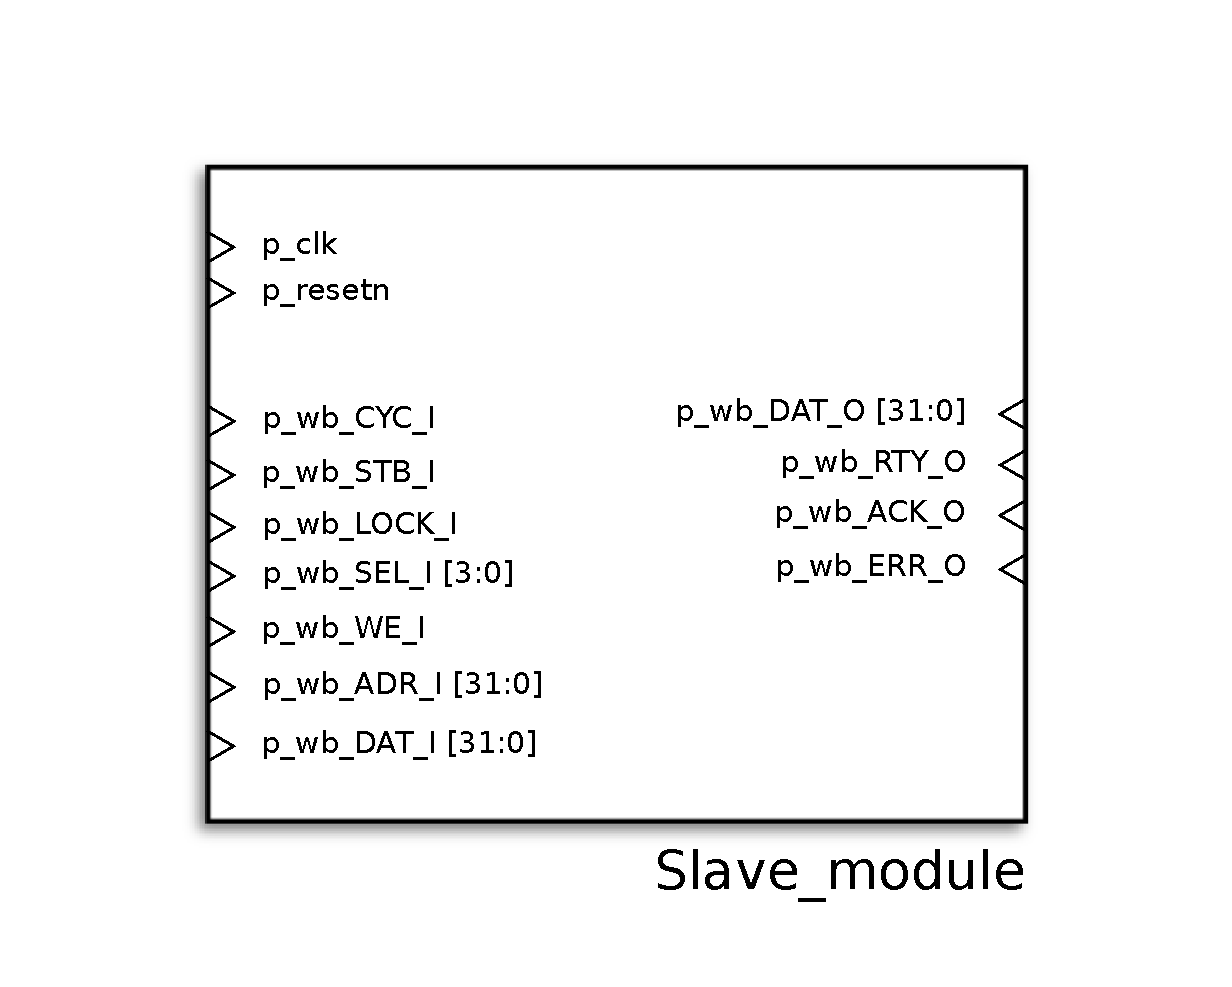
\includegraphics[width=7cm]{figs/slave_symbol.pdf}
\caption{Generic slave interface}
\label{generic_slave_interface}
\end{figure}

As several modules in our design require a slave interface to let the LM32 post to them configuration values, we decided to implement a generic slave interface, that can be easily re-used in every module.

This generic slave modules includes a state machine that handles simple read and write requests, as presented in figure \ref{state_machine_slave}.

\begin{figure}[h]
\center
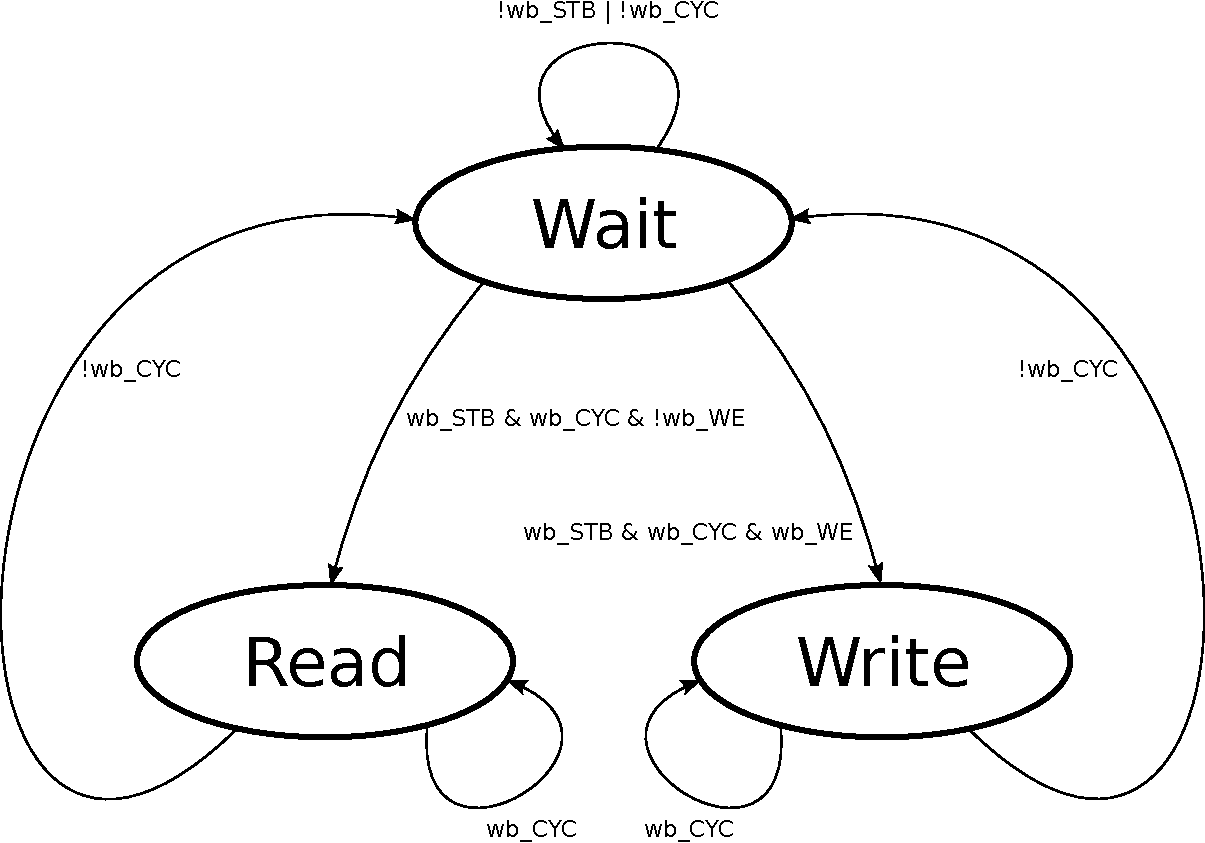
\includegraphics[width=11cm]{figs/slave_state_machine.pdf}
\caption{Generic slave's state machine}
\label{state_machine_slave}
\end{figure}

When accessing the \emph{Read} or \emph{Write} states, the module automatically calls the \texttt{slave\_read()} and \texttt{slave\_write()} methods respectively.

These methods can be overloaded in any inheriting slave interface, thus allowing a great variety of behaviors and features to rely on one single wishbone slave source code.

\paragraph{Slave module with configuration registers}
~\\~

\begin{figure}[H]
\center
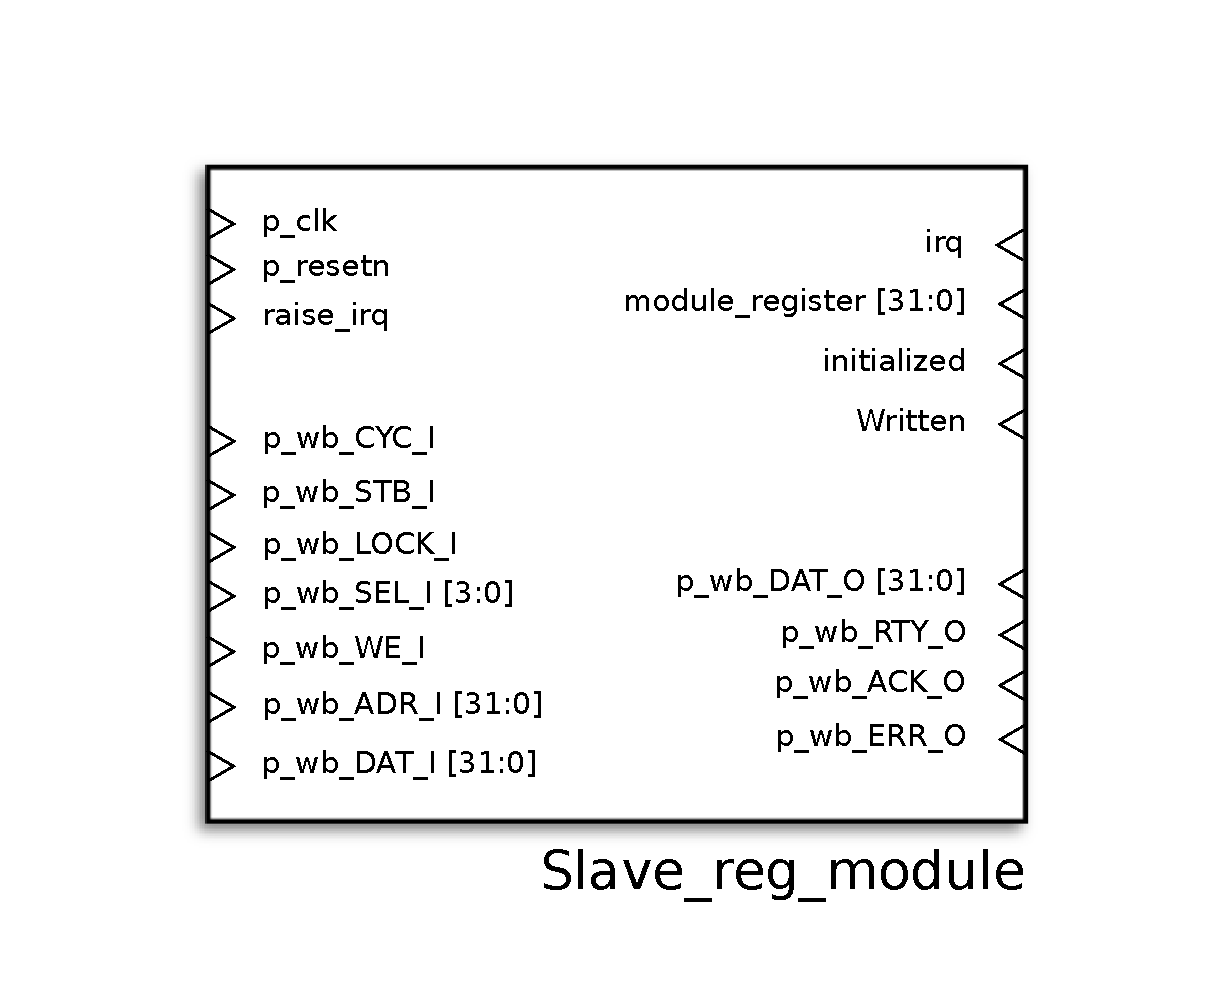
\includegraphics[width=7cm]{figs/slave_reg_hdl_symbol.pdf}
\caption{One register slave interface for use in VideoIn and VideoOut}
\label{reg_slave_interface}
\end{figure}



As we previously stated, the LM32 will configure the peripherals by writing configuration values to each slave interface.
These configuration values will be stored in internal configuration registers.

Therefore, we created slave modules that inherit the previously defined generic slave.
In addition to the generic slave module's internal components, these inheriting slave modules comprise one registers or more.
They have overloaded \texttt{slave\_read()} and \texttt{slave\_write()} which allows to transfer a write request's content to the register, as well as the register's content as an answer to a read request.

The following sections will describe the video stream modules, and how they put these slave interfaces to good use.
